% Style for a MSc paper at Warsaw School of Economics
% Michał Ramsza
% Friday, December 14, 2012

% --- document class and other global stuff ---------------------------
\documentclass[polish, twoside, 12pt, a4paper]{article}

% --- packages --------------------------------------------------------
\usepackage{textcomp}
\usepackage{times}
\usepackage{amsmath}
\usepackage{amsfonts}
\usepackage{amssymb}
\usepackage{amsthm}
\usepackage[T1]{fontenc}
\usepackage[utf8]{inputenc}
\usepackage{graphicx}
\usepackage{xcolor}
\usepackage{enumitem}
\usepackage[polish]{babel}
\usepackage[centering, left=3.5cm, right=2.5cm, textheight=24cm]{geometry}

% --- packages for citations ------------------------------------------
\usepackage{natbib}
\AtBeginDocument{\renewcommand{\harvardand}{i}}
\usepackage{ stmaryrd }

% --- package for automatic insertion of R code -----------------------
\usepackage{listings}
\lstset{language=R,%
   numbers=left,%
   tabsize=3,%
   numberstyle=\footnotesize,%
   basicstyle=\ttfamily \footnotesize \color{black},%
   escapeinside={(*@}{@*)}}

% --- support for links -----------------------------------------------	
\usepackage{url}
\usepackage{hyperref}
\hypersetup{colorlinks=true,
            linkcolor=black,
            citecolor=darkgray,
            urlcolor=darkgray,
            pagecolor=darkgray}

% --- support for large tables and other stuff ------------------------	
\usepackage{longtable}
%\usepackage{subfigure} % this package will now work with subcaption package
\usepackage{float}
\usepackage{caption}
\usepackage{subcaption}


% --- definitions for environments -------------------------------------
\theoremstyle{definition}
    \newtheorem{condition}{Assumption}
    \newtheorem{example}{Example}      

\theoremstyle{plain}
    \newtheorem{definition}{Definition}    
    \newtheorem{proposition}{Proposition}
    \newtheorem{theorem}{Theorem}
    \newtheorem{cor}{Corollary}

\theoremstyle{remark}
    \newtheorem{remark}{Remark}


%running fraction with slash - requires math mode.
\newcommand*\rfrac[2]{{}^{#1}\!/_{#2}}

% --- other settings --------------------------------------------------
\linespread{1.5}
\frenchspacing
\sloppy
\allowdisplaybreaks[4]
\raggedbottom
\clubpenalty=10000
\widowpenalty=10000

% --- only if required ------------------------------------------------
\AtBeginDocument{\renewcommand*{\figurename}{Wykres}}
\AtBeginDocument{\renewcommand*{\tablename}{Tabela}}

% ---------------------------------------------------------------------
\begin{document}

% --- strona tytulowa -------------------------------------------------
\begin{titlepage}
\centering


\includegraphics[scale= 0.6]{uw_logo.JPG}

\vspace*{0.5cm}
Studium magisterskie\\
\begin{flushleft}
Kierunek: Informatyka i Ekonometria\\
%Specjalność: Metody ilościowe w ubezpieczeniach i finansach}
Forma studiów: Stacjonarne
\end{flushleft}

\vspace*{.5cm}
\rule{0cm}{1cm}\hfill
\begin{minipage}{9cm}
Imie i nazwisko: Klaudyna Maraciniak\\
Nr albumu: 310757
\end{minipage}

\vspace*{1cm}
\begin{minipage}{12cm}
\centering
\Large
\textbf{Problem wyceny ryzyka przestrzennego - porównianie metod wygładzania danych..}
\end{minipage}

\vspace*{2cm}
\rule{0cm}{1cm}\hfill
\begin{minipage}{9cm}
Praca magisterska napisana\\
w Katedrze Statystyki i Ekonometrii\\
pod kierunkiem naukowym\\
prof. hab. Wojciecha Otto
\end{minipage}

\vfill
Warszawa, 2015
\end{titlepage}

\rule{1ex}{0ex}\clearpage

{\Large \pmb{Streszczenie} \par}

\clearpage

% --- table of contents -----------------------------------------------
\cleardoublepage
\tableofcontents

% --- chapter ---------------------------------------------------------
\cleardoublepage
\section{Wprowadzenie}
%"Działalność ubepzpieczeniowa jest jak powietrze dla gospodarki wolnorynkowej. Bez możliwosi zabezpieczenia sie przed ryzykiem finansowym czy nieszczesliwymi zdarzeniami fundamenty kapitalizmu byłyby poważnie nadwyrężone "- piszę w swoim "raporcie"  spółka AIG, podkreśłając, szczególny charakter ubezpieczeń, pelni wazna misje spoleczna i gospodarcza. Od strony operacyjnej działalność ubezpieczeniowa opiera się przede wszystkim na zarządzaniu ryzykiem. Jest ono w duzej mierze kwantyfikowalne stosuje sie modele. \\


W przypadku wielu produktów ubezpieczeniowych ryzyko ubezpieczeniowe* jest zróżnicowane przestrzennie to znaczy zależy od różnych czynnikow geograficznych? często bezpośrednio niemierzalnych lub nieobserwowalnych. 
Przykładem mogą tutaj być ubezpieczenia samochodowe. Na prawdopodobieństwo kolizji wpływają takie czynniki jak natężenie ruchu, stopień modernizacji sieci komunikacyjnej, liczba rozwiązań poprawiających bezpieczeństwo na drogach (bezkolizyjne skrzyżowania, fotoradary). W przypadku ubezpieczeń mieszkaniowych ryzyko powodzi dotyczy przede wszystkim terenów położonych w pobliżu rzek i zbiorników wodnych i istotnie zminiejsza się wraz z oddalaniem się od potencjalnego źródła powodzi. Wymienioine czynniki są związane z przestrzennym występowaniem ryzyka, dlatego naturalną reprezentacją tego probelmu powinna być funkcja, która używa jak argumentu położenia np. adresu domu lub miejsca parkowania samochodu.\\

Motywacją za tym, aby precyzyjnie wyceniać w składce przestrzenne zróżnicowanie ryzyka jest następujące. W interesie ubezpieczyciela jest poznanie możliwie dokładnie struktury swojego portfela polis tak, aby powstała taryfa uwzględniała wszystkie istotne zmienne taryfikacyjne. Oznacza to, że ubezpieczyciela będzie interesować estymacja warunkowych wartości oczekiwanych liczby i wartości szkód ze swojego portfelaj. W sytuacji, gdy ubezpieczyciel?? w warunkach konkurencji preyzyjna wycena ryzyka, chroni go przed efektem negatywnej selekcji.  Pominiecie struktury geograficznej w procesie taryfikacji, w przypadku gdy jest ona istotnym predykatorem, spowoduje napływ do portfela polis o podwyższonym ryzyku przy jednoczesnym niedoszacowaniu składek za to ryzyko, z uwagi na to że konurencja wycenia te polisy właściwie, a więc drożej. W wyniku pominiecia istotnych zmiennych taryfikacyjnych składki osób o niższym profilu ryzyka zostałbyy zawyżone, tak aby pokryć oczekiwaną wartość szkód z  całego portfela. W efekcie osoby te zdecydują się zakupić polisę w konkurencyjnym towarzystwie ubezpieczeniowym, a oczekiwany zysk ubezpieczyciela zmniejszy się. \\



Od analityka aktuarialnego wymaga to zastosowania specjalnych metod statystycznych, które pozowlą uchwycić zależności przestrzenne, a więc uzelażnić we właściwy sposób składkę od miejsca ubezpieczenia. Chcąc ustalić jaki wpływ ma na pewne zjawisko efekt przestrzenny, wpierw należy przeprowadzić estymacje modelu, bez użycia zmiennych o charakterze przestrzennym. Porównanie rzeczywistej liczby szkód z westymowanymi wartościami daje pojęcie o tym jak efekt przestrzenny wpływa na oczekiwaną częstość szkód w różnych regionach.  Powstaje jednak problem związany z faktem, że do estymacji modelu została użyta losowa próba (portfel polis, którym dysponował z pewnego przkeroju czasu ubezpieczyciel), w rezultacie oszacowany efekt przestrzenny jest obarczony błedę estymacji wynikjącym z wariancji składnika losowego. Problem wariancji danych ma dwojaki charakter. Na wariancje ma wpływ faktyczne zróżnicowanie przestrzenne ryzka jak także fakt, iż otrzymane częstości są "jedynie" średnią z próby, a prawdziwa wartość oczekiwana czestości szkód nie jest znana. Wymaga to zastosowania dodatkowych metod staytsycznych, aby "odszumić" underlyaing spatial sygnał .
\\


%* nie karac dwa razy za to samo \\
%* ryzyko jako zmienna losowa wyrazona w jednostkach pienieznych\\


Należy się zastanowić jaka forma danych będzie adekwatna, aby reprezentować położenie, w szczeglności jaki poziom granulacji danych powinnnien zotać zastosowany . Funkcja opisująca ryzyko przestrzenne przeważnie jest miejscami nieciągłą, a znaczna część dzieniny tej funkcja jest funkcją gładka(na pewnych przedziałach). Istnieją jednak przesłanki za tym, aby zależności przestrzenne prezentować w podziale na poligony (np. mapa kodów pocztowych) niż za pomocą  gładkiej płaszczyzny.???
Z drugiej jednak strony należy mieć na uwadzę realane ograniczenia ubezpieczyciela w postaci  jakości i granulacji danych jakimi dysponuje. W przypadku położenie najczęściej będzie to przybliżona informacja o lokalizacji np. kod pocztowy, rzadziej punkt w pewnym układzie współżednych(np. współrzędne geograficzne). Z praktycznego punktu powiązanie ryzyka geograficznego ze składką za ubezpieczenie za pomocą kodów pocztowych wydaje się mięć wiekszę zastosowanie w praktyce ubezpieczeniowej.


 Literatura prezentująca metody estymacji ryzyka geograficznego, której rezultatem jest przyporządkowanie kodom pocztowym wyestymowanego ryzyka, nie jest obszerna. I:\\a
*\\
* ..\\

W wcześniejszych publikacjach dotyczących można wyróżnić dwa podejścią estymacji ryzyka geograficznego. Krok pierwszy jest taki sam w obu przypadkach.  


1. Dane surowe obrazujące "ryzyko przestrzenne" otrzymane po estymacji modelu muszą zostać wygładzone w stopniu który maksymalnie ograniczy wariancje o charakterze losowym \pmb{jak to sie nazywa po polsku} .  \\
2. Interesujące nas dane najpierw posłużą do utworzenia w oparciu o kody pocztowe regionów ratingowych, według nastepujących kryterium: 

a)Przy pozosta parametrach stalych składka nie powinna różnić się na obszarze danego regionu ratingowego, \\

b)jednocześnie składki w różnych regionach różnia się pod względem \pmb{premii za ryzyko geograficzne}.\\


W niniejszej pracy zostało zastosowane podejście pierwsze w którym należy wygładzić reszty otrzymany z modelu regresji, dla rozpatrywanych poligonów, tak aby usunąć wpływ czynników losowych na wartość estymowanej zmiennej.
(w ninejszej pracy zakładamy multiplikatywna zalezność pomiedzy czynnikami przestrzennymi a pozostałymi czynikami mającymi wpływ na warunkową watość oczekiwaną częstości szkód) \\
%i które ze względu na to jak przebiega podział administracyjny Polski (ta sama gmina ma te same pierwsze cyfry kodu pocztowego). gsghsrkg'

- w ninejszej pracy estymacja efektu przestrzennego została przeprowadzona dla częstości szkód - 



\clearpage
\section{Układ treści}	
Wprowadzenie zawiera informacje o 
W rozdziale drugim została omówiona literaturą która dotyczy jak również



\clearpage
\section{Literatura przedmiotu}


% --- chapter ---------------------------------------------------------
\clearpage
\section{Teoria}
\subsection{Założenia teoretyczne}
Przedstawiona w dalszej części pracy metodologia wygładzania czynnika przestrzennego wymaga przyjęcia pewnych założeń dotyczących relacji między rozpatrywaną zmienną (np. częstość szkód) a czynnikiem geograficznym, który warunkuje rozkład tej zmiennej. Interesje nasz w szczególnośći jak wpływa on na warunkową wartość oczekiwaną i wariancję.\\

 
Rozważmy zmienną losową \(Y\), której średnia \(\mu_{ijk}\) zależy od \(n\) zmiennych. \(N\) może być dowolną liczbą naturalną jednak dla uproszczenia poniższe przekształcenia zostaną przedstawione dla \(n=3\),  na przykładzie zmiennych \(X_1\), \(X_2\), \(X_3\). Zmienna \(X_3\) opisuje położenie obserwacji za pomocą współrzędnych kartezjańskich w \(R^2:\)  \(\boldsymbol{X_3}=(x_1,x_2)\).
Niech indeksy \(i\),\(j\),\(k= 1,2,3..\)  oznaczaja poszczególne podzbiory obserwacji wydzielone ze względu na  przyjmowane wartości  przez zdyskretyzowane zmienne \(X_1\), \(X_2\), \(X_3\). \\
Obserwacje można przedstawić jako strukturę/komórkę danych \({Y_{ijk}, N_{ijk}}\) - gdzie \(Y_{ijk}\) oznacza  zmienną objaśnianą a  \(N_{ijk}\) jest miarą (ang. exposure). Taką strukturę reprezentuje przeważnie kilka polis z portfela ubezpieczyciela, które mają taką same wartości zmiennych $X_2$, $X_3$ i pochodzą z tego samego obszaru.\\



Na przykładzie tej pracy zmienna losowa $Y_{ijk}$ jest częstością szkód dla i-tego kodu pocztowego, j-tej wartości zmiennej $X_2$ i k-tej wartości zmiennej $X_3$. Zmienna $X_1$ oznacza centroid kodu pocztowego a $N_{ijk}$ to liczba lat życia polisy w ciagu rozważanego okresu czasu.   

Wartość oczekiwana $Y_{ijk}$ na jest wyrażona przez $\mu_{ijk}$:

\[
E[Y_{ijk}]=\mu_{ijk}.
\]

Zakładając, że efekt przestrzenny jest niezależny od pozostałych czynników warunkujących średnią \(\mu_{ijk}\), można zapisać poniższe:

\[
\mu_{ijk}=v_i \theta_{jk}
\]

Gdzie \(v_i\)  to składowa średniej  \(\mu_{ijk}\) wyodrębniająca efekt przestrzeny a \(\theta_{jk}\) to składowa reprezentująca pozostałę czynniki od których zależy średnia. Wartości \(\theta_{jk}\) zostały wyestymowane np. przy użyciu uogólninego modelu liniowego (ang. general linear model). Zdefinujmy $\bar{Y_i}$ jako :

\[
\bar{Y_i}=\cfrac{\sum\limits_{jk} N_{ijk} (\frac{X_{ijk}}{\theta{ijk}})}{\sum\limits_{jk} N_{ijk}}
\] \\[0.00001pt]
$\bar{Y_i}$  to oczekiwane prwadopodobieństwo wystąpienia szkody, za które odpowiada efekt przestrzenny \(v_i\), wyestymowane na podstawie dostępnej próby. 
Zatem wartość oczekiwana \(\bar{Y_i}\) wyodrębnia efekt przestrzenny:

\[
E[\bar{Y_{i}}]=v_{i}.
\]\\[0.00001pt] Dodatkowo przyjmijmy założenie dotyczace wariancji, że dla pewniego $\sigma^2 > 0$  zachodzi:

\[
Var[\bar{Y_{i}}]=\frac{\sigma^2}{N_i}
\]


gdzie,

\[
N_i=\sum\limits_{jk}{N_{ijk}}
\]\\[0.00001pt]
Jeśli zmienne losowe $Y_{ijk}$ i $X_{ijk}$ mają rozkład prawdopodobieństwa Poissona, wtedy ich wartość oczekiwana i wariancja są sobie równe, więc wariancja zależy w następujący sposób od $v_{i}$:

\[
Var[\bar{Y_{i}}]=\frac{\phi_{i} v_i}{N_i}
\]

Z własności rozkładu Poissona $\phi_{i}$ można zapisać jako:

\[
\phi_{i}=\sum\limits_{jk}(N_{ijk}/N_{i})\theta^{-1}_{jk}
\]

Oczywiśćie \(v_{i}: R^2 \shortrightarrow R\) i \(\bar{Y_{i}}: R^2 \shortrightarrow R\)  zależa od współrzednych na płaszczyźnie euklidesowej:


\[
v_{i} = v(\boldsymbol{x_i})
\]


\[
\bar{Y_{i}} = \bar{Y}(\boldsymbol{x_i}).
\]




\clearpage
\subsection{Model wygładzania Whittakera}

Rozważmy punkty \(x \in R^2\) w dwuwymiarowej przestrzeni euklidesowej. Zadany problem optymalizacyjny polega na znalezieniu współczynników funkcji \(W (y):R \shortrightarrow R^2 \) poprzez dopasowanie współczynników wielomianów rzędu co najwyżej drugiego.


\[
Q_{x}(y) = q^T_x y^{\otimes}.
\]


gdzie \(y=(y_1,y_2)^T\) oraz

\[
y^{\otimes}=(\frac{1}{2}y_1^2, y_1y_2, \frac{1}{2}y_2^2, y_1, y_2, 1)^T,
\]

gdzie \(q_x\) jest wektorem współczynników wielomianu \(Q_x\)


Niech \(y_x^{(1)}, y_x^{(2)}, ... , y_x^{(h)}\) będzie zbiorem najbliższych $h$ punktów do \(x\), gdzie \(y_x^{(1)} = x\)    


\[
z_x=[W(y_x^{(1)}), W(y_x^{(2)}), ...   , W(y_x^{(h)})]^T .
\]



\[
q_x= A_x z_x,
\]


\[
A_x = (X_x^TX_x)^{-1}X_x^T
\]

Elementy wektora  \(q_x\) to współczynniki wielomianu kwadratowego dopasowanego do h punktów w przestrzeni \(R^3\). Otrzymano w ten sposób płaszczyznę loklanie odwzorujacą otoczenie punktu \(x\). Jest to wielomian najniższego stopnia dla którego możliwe jest policzenie pochodnej drugiego rzedu. Należy teraz wyrazić w kontekście calego zbioru m punktów: \(z=[W(x_1), W(x_2), ...   , W(m)]\). Elementy wektora  \(q_x\) posłużą do zbudowania macierzy \(A_x\), która pozwoli na optymalizacje współczynników \(W(x)\) na całym rozważanym przez nas obszarze. Uogólnienie na całą optymalizowaną płaszczyznę otrzymujemy poprzez:  

\[
 q_x=B_x z_x,
\]



\[
 \bar{q}_x=\bar{B}_x z_x,
\]

drugi człon funkcji kary, będący miarą wygładzenia funkcji:

\[
 S(x)=\tilde{q}_x^T C \tilde{q}_x
\]

gdzie macierz \(C\) to następująca macierz diagonalna:

\[
C=
\begin{bmatrix}
1                & 0 & 0       \\
0                & 2 & 0  \\
0		& 0 & 1
\end{bmatrix}
\]


\[
 S(x)=z^T \tilde{B}_x^TC\tilde{B}_xz,
\]

\[
S=z^T [\sum\limits_{i}{\tilde{B}_{x_{i}}^TC\tilde{B}_{x_{i}}]}z.
\]

\clearpage
\subsection{Model cienkiej płytki}

Model cienkiej płytki (ang. thin plate spline) 



 Introduction. Radial basis functions (RBFs) have emerged as one powerful
tool for scattered data approximation in high dimensional space. They have been
successfully applied in various applications including
· geography and digital terrain modelling [23][24][25];
· data assimilation in geodesy and metrology [39][17];
· engineering design and mesh generation [28][29] [35]


radialna funkcja bazowa to\;

\[
y(\boldsymbol{x})=\sum\limits_{k}{w_k\rho(||\boldsymbol{x-x_k}||)}
\]

\[
y_k=\sum\limits_{l}^{K}{w_l\rho_{lk}}
\]

gdzie \(y(\boldsymbol{x_k})=y_k\) to znane wartosci aproksymacyjne


\[
\begin{bmatrix}
y_1 \\ y_2 \\ ... \\ y_K
\end{bmatrix}
=
\begin{bmatrix}
\rho_{11} &  \rho{12} & ... & ... \\
\rho_{21} & ... & ... & ... \\
... & ... & ... & \rho_{KK} 
\end{bmatrix}
\begin{bmatrix}
w_1 \\ w_2 \\ ... \\ w_K
\end{bmatrix}
\]

radialna funckja bazowa cienkiej płytki:

\[
\rho(r) = r^2log(r)
\]

radialna funkcja bazowa Wendlanda:

\[
\rho(r) =
\left\{
\begin{aligned}
(1-\frac{r}{R})^4 (4 \frac{r}{R}+1) &\quad  dla  &\quad \frac{r}{R} < 1 \\
0 &\quad dla &\quad  \frac{r}{R} \geq 1
\end{aligned}
\right.
\]


\clearpage
\section{Postać i przekształcenia danych}






\clearpage

\clearpage
\section{Rysunki i tablice}

Zarówno rysunki jak i tablice używają podobnej koncepcji osadzania w dokumencie. Aby osadzić tablicę używa się otoczenia  \verb+table+. Poniżej jest przykład prostej tablicy.

\begin{table}[hbt]
  \centering

  \captionsetup{margin=10pt,font=small,labelfont=bf,width=.8\textwidth}

  \caption[Przykład prostej tablicy]{Przykład prostej tablicy. Ten tekst będzie automatycznie zawijany. \textit{Źródło:} opracowanie własne.}
  \label{tab:exceptional-table}

\vspace*{2ex}

  \begin{tabular}{lccc}
    Name        & property 1 & property 2 & property 3 \\ \hline
    Michael     & 23         & 34         & --         \\
    John        & 34         & --         & 28         \\
    Mr. Niceguy & 123        & 231        & 312        \\ \hline
  \end{tabular}
\end{table}

Tablica~\ref{tab:exceptional-table} jest przykładem bardzo prostej tablicy ale możliwe jest znacznie więcej rzeczy, w razie konieczność służę pomocą.

Aby osadzić rysunek to w pierwszej kolejności trzeba mieć ten rysunek w pliku. W katalogu są dwa przykładowe rysunki. Następujący przykład korzysta z tych rysunków i jest przykładem wykorzystania otoczenia \verb+figure+.

\begin{figure}[hbt]
  \centering

  \begin{subfigure}[t]{0.45\textwidth}
    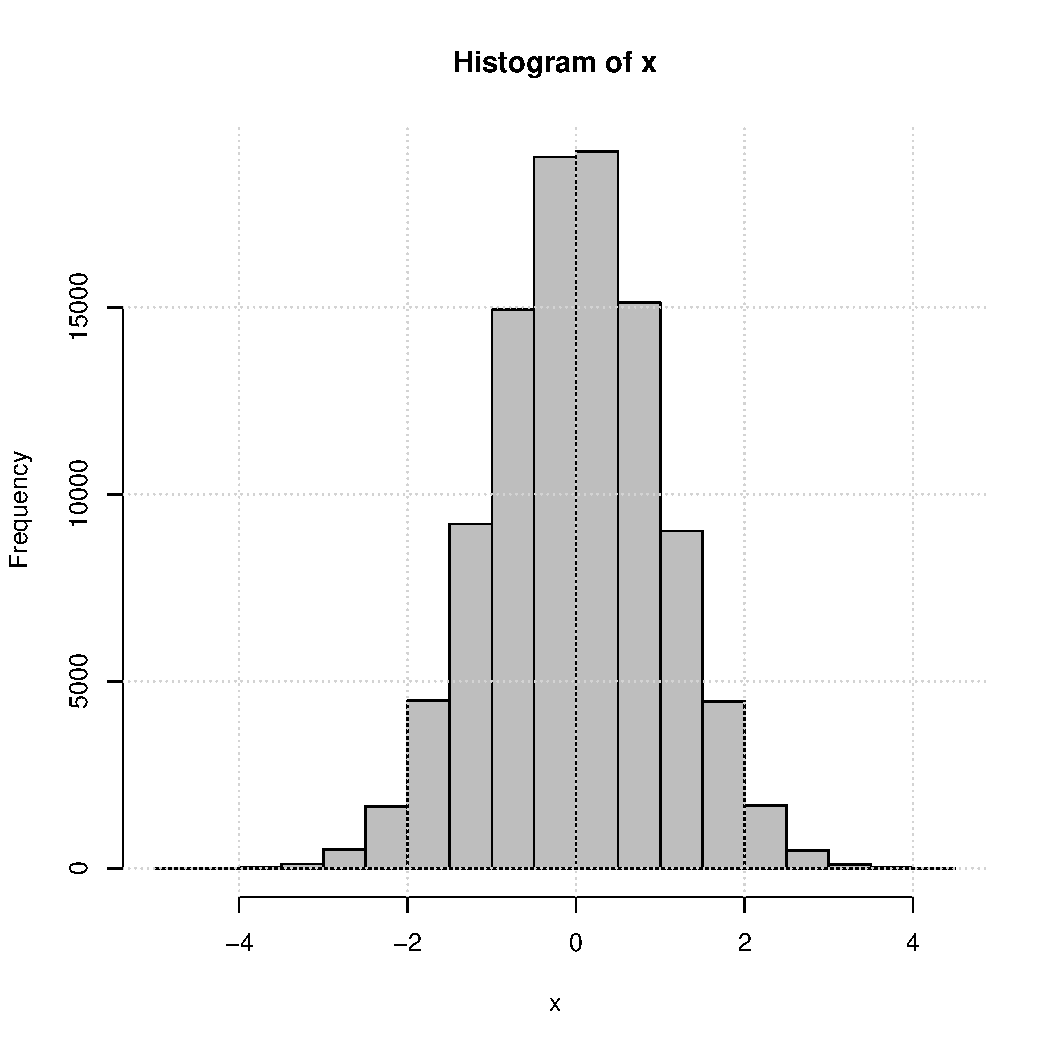
\includegraphics[width=\textwidth]{./figure-1}
  \end{subfigure}

  \captionsetup{margin=10pt,font=small,labelfont=bf,width=.8\textwidth}

  \caption[Krótka nazwa X]{Przykładowy pojedynczy wykres. \textit{Źródło:} opracowanie własne}\label{fig:xxx1}
\end{figure}

\begin{figure}[hbt]
  \centering
  \begin{subfigure}[t]{0.45\textwidth}
    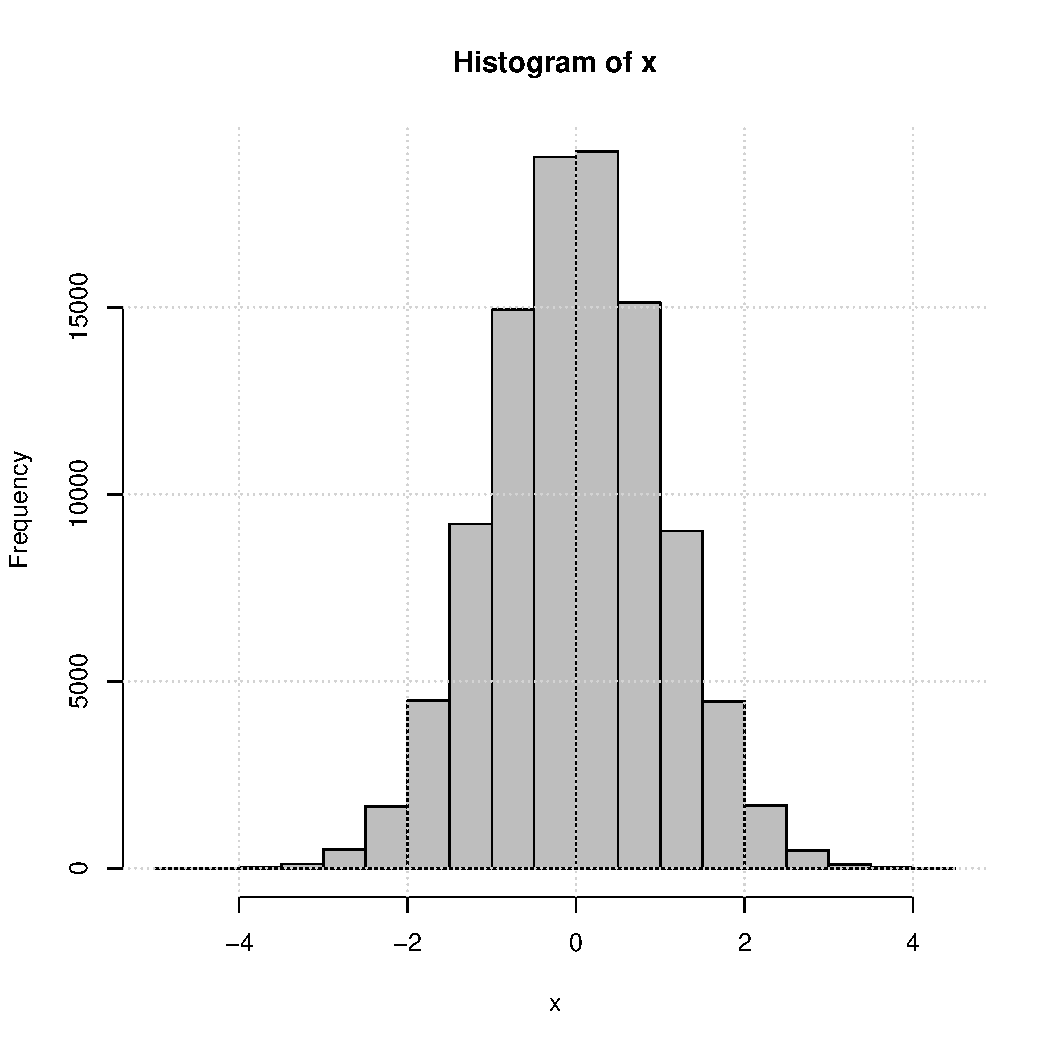
\includegraphics[width=\textwidth]{./figure-1}
    \caption{To jest pierwszy podpis. Ten podpis będzie również zawijany ale będzie to powodowało odpowiednie dopasowanie wysokości.}
    \label{fig:xxxa}
  \end{subfigure}
  \hfill
  \begin{subfigure}[t]{0.45\textwidth}
    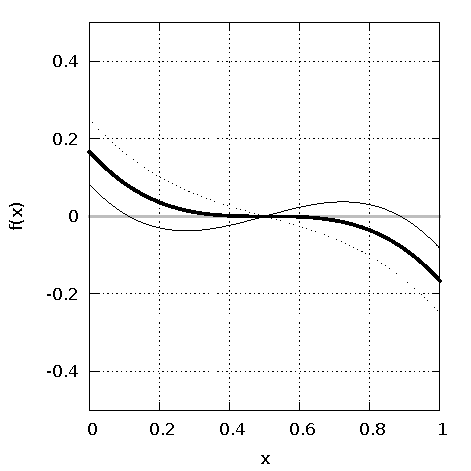
\includegraphics[width=\textwidth]{figure-2}
    \caption{Układ równowag stabilnych}
    \label{fig:xxxb}
  \end{subfigure}
  
  \captionsetup{margin=10pt,font=small,labelfont=bf,width=.8\textwidth}

  \caption[Krótka nazwa II]{Przykładowy wykres. Wykresy podpisujemy, a więc ten opis znajduje się pod wykresem. \textit{Źródło:} opracowanie własne}\label{fig:xxx}
\end{figure}



Odwołanie się do wykresu działa podobnie jak do równania: rysunek~\ref{fig:xxx1}. Możemy również odwoływać się do podwykresów:~\ref{fig:xxxa} lub \ref{fig:xxxb}. Zarówno tablice (tabele) jak i rysunki (wykresy) są automatycznie układane przez \LaTeX{} i nie pozycjinujemy ich sami.

% --- chapter ---------------------------------------------------------
\clearpage
\section{Literatura}

Zawartość literatury znajduje się w innym pliku o nazwie \verb+refs.bib+. Mogą Państwo zmienić nazwę tego pliku ale wtedy trzeba również zmienić w tym pliku informację z \verb+\bibliography{refs}+ na \verb+\bibliography{new-name}+ gdzie \verb+new-name+ jest nazwą nowego pliku z literaturą. Załączony plik  \verb+refs.bib+ zawiera przykłady cytowań dla książek i artykułów. 

Sam proces cytowania jest prosty. Używa się komendy \verb+\cite{garland2010}+, która wygeneruje odpowiednie cytowanie \cite{garland2010} oraz dołączy odpowiednią informację na końcu dokumentu.Wszystko jest automatycznie sortowane i formatowane więc nie ma potrzeby zajmowania się tym ręcznie. Przykłady cytowania artykułów z wieloma autorami: \cite{benaim2003}, \cite{osborne1998}. 


% --- appendices ------------------------------------------------------
\appendix

% ---------------------------------------------------------------------
\clearpage
\section{Dodatek: Ważne rzeczy do dodania}

Tutaj można włożyć długie tablice, kod wykorzystane w pracy lub inne elementy, które nie powinny zakłócać czytania tekstu.


% --- bibliography ----------------------------------------------------
\clearpage
www.aig.com/aigweb/internet/en/files/AIG\%20Systemic\%20Risk2\_tcm385-152209.pdf \newline
A Guide to Insurance: Combining Governance, Compliance and Regulation: Nigel Feetham,Robin Amos \\
Przestrzenne zróżnicowanie ryzyka ubezpieczeniowego a efektywność ubezpieczeń na życie : ryzyko - popyt - zysk / Adam Śliwiński. \\
Geographic Variation in Premiums in Helath insurances Marketplaces RUPRI \\


\bibliographystyle{agsm}
\bibliography{refs}

% --- abstract --------------------------------------------------------
\clearpage
\addcontentsline{toc}{section}{Lista tablic}
\listoftables

% --- abstract --------------------------------------------------------
\clearpage
\addcontentsline{toc}{section}{Lista rysunków}
\listoffigures



% --- abstract --------------------------------------------------------
\clearpage
\addcontentsline{toc}{section}{Streszczenie}
\section*{Streszczenie}

Tutaj zamieszczają Państwo streszczenie pracy. Streszczenie powinno być długości około pół strony.


\end{document}

